

\documentclass[11pt, a4paper]{report}

\usepackage[utf8]{inputenc}


\usepackage{hyperref}


\usepackage[a4paper, total={6in, 8in}]{geometry}

\usepackage{algorithm}
\usepackage{algpseudocode}

\usepackage{ragged2e} %--For text alignment

\newenvironment{frontmatter}{}{\maketitle}

\usepackage{longtable}

\usepackage{graphicx}
\usepackage{rotating}
\usepackage{amssymb,amsmath}
%% The lineno packages adds line numbers. Start line numbering with
%% \begin{linenumbers}, end it with \end{linenumbers}. Or switch it on
%% for the whole article with \linenumbers after \end{frontmatter}.
%\usepackage{lineno}
\newtheorem{theorem}{Definition}
\usepackage{subfigure}
\usepackage{lscape}
\usepackage{etoolbox}
\usepackage{xstring}
\usepackage{textcomp}
\usepackage{rotating}
\usepackage{booktabs}
\usepackage{siunitx}

%\usepackage{datetime}

%\usepackage{fancyhdr}
% 
%\pagestyle{fancy}
%\fancyhf{}
%\rhead{Put your tit}
%\lhead{Title}
%\rfoot{Page \thepage}

% Enter Details about your project here
\newcommand{\ProjectTitle}{Regression Analysis using Swarm Intelligence}
\newcommand{\AuthorName}{Arkanayan Shit}
\newcommand{\SupervisorName}{Tapas Si}
% Leave unchanged if you don't have co-supervisor
\newcommand{\CoSupervisorName}{Asim Kumar Mahadani}
\newcommand{\HODName}{Aloke Roy}

\begin{document}

\begin{titlepage}
    \begin{center}
        \vspace*{0.01cm}
        \huge
        \textbf{\ProjectTitle}
        
        
        \vspace{1.5cm}
        
        Submitted by\\
        \textbf{\AuthorName}
         
         University Roll No.10500113001         
        
        \vfill
        
        A project report  submitted in partial fulfillment for the degree of
       Bachelor of Technology in Computer Science \& Engineering
        
        \vspace{0.8cm}
        
        
\includegraphics[width=0.4\textwidth]{buie_logo.jpg}
        
        Department Computer Science \& Engineering\\
        Bankura Unnayani Institute of Engineering\\
        Bankura - 722 146, West Bengal, India\\
       
       {January}{\hspace*{0.5cm}}{2017}
       %\date{\displaydate{date}}
        
    \end{center}
\end{titlepage}
\newpage

\pagenumbering{gobble} 

\begin{center}
\vspace*{8.5cm}
\LARGE
\textit{Dedicated to my parents}

\end{center}



\newpage
{\it ``We are what our thoughts have made us; so take care about what you think. Words are secondary. Thoughts live; they travel far.''}
\begin{flushright}
- Swami Vivekananda
\end{flushright}


{\it ``Take up one idea. Make that one idea your life - think of it, dream of it, live on that idea. Let the brain, muscles, nerves, every part of your body, be full of that idea, and just leave every other idea alone. This is the way to success.''\\}

\begin{flushright}
- Swami Vivekananda
\end{flushright}

{\it ``When an idea exclusively occupies the mind, it is transformed into an actual physical or mental state.''}
\begin{flushright}
- Swami Vivekananda
\end{flushright}

{\it ``You have to dream before your dreams can come true.''}
\begin{flushright}
-Dr. A. P. J. Abdul Kalam
\end{flushright}


{\it ``Dream is not that which you see while sleeping it is something that does not let you sleep.''}
\begin{flushright}
-Dr. A. P. J. Abdul Kalam
\end{flushright}

\newpage


 \begin{center}
        \vspace*{1cm}
         \LARGE
        \textbf{Certificate of Approval}
        
        \vspace{1.5cm}
 \justify      
		The forgoing project report is hereby approved as a creditable study of Technological subject carried out and presented in a manner satisfactory to warrant its acceptance as a prerequisite with degree for which it has been submitted. It is to be understood that by this approval, the undersigned do not necessarily endorse or approve any statement made, opinion expressed or conclusion drawn there in but approve the thesis only for the purpose for which it has been submitted.        
        
        \vspace{1.5cm}
        
        Board of Examiners
        
        \begin{itemize}
        \item 
        \item
        \item
        \item
        \end{itemize}
        
        \vfill
        
       
        
        
        
    \end{center}

\newpage


\begin{center}
        \vspace*{1cm}
         \LARGE
        \textbf{Declaration}
        
        \vspace{1.5cm}
 \justify      
		I hereby declare that this submission is my own work and that, to the best of my knowledge and belief, it contains no material previously published or written by another person nor material which has been accepted for the award of any other degrees or diplomas of the university or other institutes of higher learning, except which due acknowledgment has been made in this text.         
        
        \vspace{5.5cm}
        
  \begin{flushleft}
   ...............................................\\
      \hspace{2.5cm}Signature
\end{flushleft}        
      
 
        
        \vfill
        
       
        
        
        
    \end{center}



\newpage
\begin{center}
        \vspace*{1cm}
         \LARGE
        \textbf{Certificate}
        
        \vspace{1.5cm}
 \justify      
		This is certified that the work contained in this report entitled, \ProjectTitle, by \AuthorName, has been carried out under the supervision of the undersign and this work has not been submitted elsewhere for any other degree.       
        
        \vspace{2.5cm}
 \small       
  \begin{flushleft}
(Signature of the Supervisor)\\
Mr. \SupervisorName, Assistant Professor, Department of CSE\\
Bankura Unnayani Institute of Engineering\\
Bankura, West Bengal

\vspace{1.5cm}

% If you have co supervisor, then only it will show
\IfStrEq{\CoSupervisorName}{CoSupervisorName} {

}{
	(Signature of the Co-supervisor)\\
	Mr. \CoSupervisorName, Assistant Professor, Department of CSE\\
	Bankura Unnayani Institute of Engineering\\
	Bankura, West Bengal
}


\vspace{1.5cm}

(Signature of the HoD)\\
Mr. \HODName, Associate Professor, Department of CSE\\
Bankura Unnayani Institute of Engineering\\
Bankura, West Bengal


\end{flushleft}        
      
 
        
        \vfill
        
       
        
        
        
    \end{center}
\newpage

\begin{center}
        \vspace*{1cm}
         \LARGE
        \textbf{Acknowledgments}
        
        \vspace{1.5cm}
 \justify      
		I hereby wish to express my sincere gratitude and respect to Assistant Prof. \SupervisorName, Dept. of CSE, Bankura Unnayani Institute Of Engineering, Bankura under whom I had proud privilege to work. His valuable guidance and encouragement have really led me to the path of completion of this project. Any amount of thanks would not be enough for the valuable guidance of my supervisor. 
I would also like to thank all the faculty member of CSE dept. for their devoted help. I also cordially thank all laboratory assistants for their cooperation.
Finally, I would like to pen down my gratitude towards my family members for their continuous support and encouragement. It would have not been possible to complete my work without their support.
   
        
     
        
        \vfill
        
       
        
        
        
    \end{center}
    


\newpage
\vspace*{1cm}
\begin{center}
\LARGE
\textbf{Abstract}
\end{center}

\justify
Regression analysis is a form of predictive modelling technique which investigates the relationship between a dependent (target) and independent variable (s) (predictor). A large part of Regression analysis deals with optimization problems. Optimization is finding the optimum (maximum or minimum) value of a co-efficients for which a function has minimum difference between predicted value and real value. Some optimization algorithms are Gradient Descent, Particle Swarm Optimization, Differential Evolution, Fireworks algorithm.

 
 \vspace*{1cm}
 \smallskip
\noindent \textbf{Keywords.} Regression analysis, Gradient Descent, Particle Swarm Optimization, Differential Evolution, Fireworks algorithm

 

\newpage
%\addcontentsline{toc}{chapter}{*}
\tableofcontents



\listoffigures


\newpage

\listoftables

\newpage
%\setcounter{page}{1}
\pagenumbering{arabic}
\chapter{Introduction}
%\justify
Regression analysis is a form of predictive modelling technique which investigates the relationship between a dependent (target) and independent variable (s) (predictor). This technique is used for forecasting, time series modelling and finding the causal effect relationship between the variables. For example, relationship between rash driving and number of road accidents by a driver is best studied through regression. 
\\

Regression analysis is an important tool for modelling and analyzing data. Here, we fit a curve / line to the data points, in such a manner that the differences between the distances of data points from the curve or line is minimized.  \cite{desc:RegressionAnalysis}
\\
\begin{figure}[!bth]
	\center
	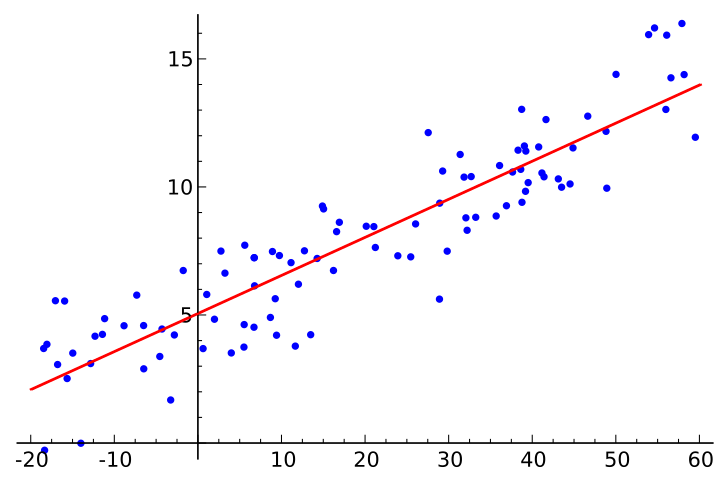
\includegraphics[scale=0.6]{images/Linear_regression}
	\caption[Regression Analysis]{Regression Analysis \cite{wiki:LinearRegression}}
	\label{fig:regressionanalysis}

\end{figure}
	

\newpage

\chapter{Background Theory}

%{\LARGE Types of Regression Techniques}

\section*{Types of Regression Techniques}

\section{Linear Regression}

It is one of the most widely known modeling technique. Linear regression is usually among the first few topics which people pick while learning predictive modeling. In this technique, the dependent variable is continuous, independent variable(s) can be continuous or discrete, and nature of regression line is linear. \\

Linear Regression establishes a relationship between dependent variable (Y) and one or more independent variables (X) using a best fit straight line (also known as regression line). \\

It is represented by an equation $ Y=a+bX + e $ , where a is intercept, b is slope of the line and e is error term. This equation can be used to predict the value of target variable based on given predictor variable(s).

\begin{figure}[!bth]
	\center
	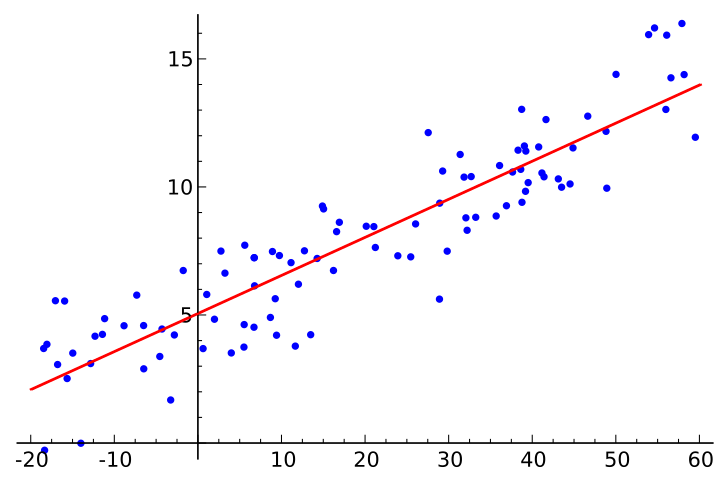
\includegraphics[scale=0.4]{images/Linear_regression}
	\caption[Linear Regression]{Linear Regression \cite{wiki:LinearRegression}}
	\label{fig:linearRegression}
\end{figure}

The difference between simple linear regression and multiple linear regression is that, multiple linear regression has (\textgreater1) independent variables, whereas simple linear regression has only 1 independent variable. \cite{desc:RegressionAnalysis} 


\section{Logistic Regression}

Logistic regression is used to find the probability of event=Success and event=Failure. We should use logistic regression when the dependent variable is binary (0/ 1, True/ False, Yes/ No) in nature. Here the value of Y ranges from 0 to 1 and it can represented by following equation.


\[ odds = \frac{p}{(1-p)} = \frac{probability \ of event \ occurrence}{probability \ of \ not \ event \ occurrence}
\]
\[ \ln{odds}  = \ln{\frac{p}{(1-p)}} \]


\[ logit (p) = \ln{\frac{p}{(1-p)}} \]

Above, \textit{p} is the probability of presence of the characteristic of interest. A question that you should ask here is "why have we used log in the equation?". \\

Since we are working here with a binomial distribution (dependent variable), we need to choose a link function which is best suited for this distribution. And, it is \href{https://en.wikipedia.org/wiki/Logistic_function}{\textit{logit}} 
function. In the equation above, the parameters are chosen to maximize the likelihood of observing the sample values rather than minimizing the sum of squared errors (like in ordinary regression). \cite{desc:RegressionAnalysis}

\begin{figure}[!bth]
	\center
	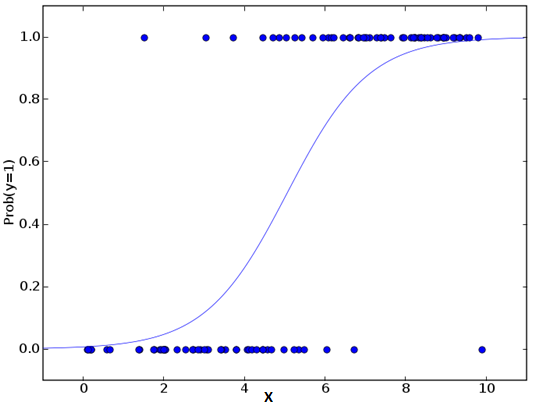
\includegraphics[scale=0.5]{images/Logistic_Regression.png}
	\caption[Logistic Regression]{Logistic Regression \cite{desc:RegressionAnalysis}}
	\label{fig:logisticRegression}
\end{figure}


\section{Polynomial Regression}

A regression equation is a polynomial regression equation if the power of independent variable is more than 1. The equation below represents a polynomial equation:

\[ y=a+bx^2 \]

In this regression technique, the best fit line is not a straight line. It is rather a curve that fits into the data points. \cite{desc:RegressionAnalysis}

\begin{figure}[!bth]
	\center
	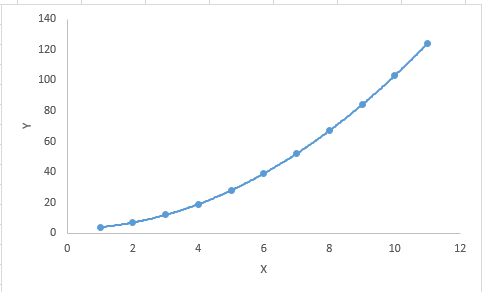
\includegraphics[scale=0.4]{images/Polynomial.png}
	\caption[Polynomial Regression]{Polynomial Regression \cite{desc:RegressionAnalysis}}
	\label{fig:ploynomialRegression}
\end{figure}

\subsection{Important Points}

\begin{itemize}
	\item {While there might be a temptation to fit a higher degree polynomial to get lower error, this can result in over-fitting. Always plot the relationships to see the fit and focus on making sure that the curve fits the nature of the problem. Here is an example of how plotting can help: 
%		\begin{itemize}
				\begin{figure}[!bth]
				\center
				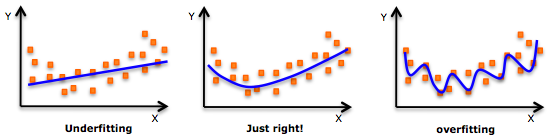
\includegraphics[scale=0.6]{images/underfitting-overfitting.png}
				\caption[Underfitting \& Overfitting]{Underfitting \& Overfitting \cite{desc:RegressionAnalysis}}
				\label{fig:underfittingOverfitting}
			\end{figure}
%		\end{itemize}

	}
	\item Especially look out for curve towards the ends and see whether those shapes and trends make sense. Higher polynomials can end up producing wierd results on extrapolation. \cite{desc:RegressionAnalysis}
\end{itemize}

\section{Applications of Regression Analysis}

Regression analysis estimates the relationship between two or more variables. Let’s understand this with an easy example: \\

Let\textquotesingle s say, you want to estimate growth in sales of a company based on current economic conditions. You have the recent company data which indicates that the growth in sales is around two and a half times the growth in the economy. Using this insight, we can predict future sales of the company based on current \& past information. \\

There are multiple benefits of using regression analysis. They are as follows:

\begin{itemize}
	\item It indicates the significant relationships between dependent variable and independent variable.
	
	\item It indicates the strength of impact of multiple independent variables on a dependent variable.
\end{itemize}

\subsubsection{Predicting the Future}
The most common use of regression in business is to predict events that have yet to occur. Demand analysis, for example, predicts how many units consumers will purchase. Many other key parameters other than demand are dependent variables in regression models, however. Predicting the number of shoppers who will pass in front of a particular billboard or the number of viewers who will watch the Super Bowl may help management assess what to pay for an advertisement. Insurance companies heavily rely on regression analysis to estimate how many policy holders will be involved in accidents or be victims of burglaries, for example. \cite{desc:RegressionApplication}

\subsubsection{Optimization}
Another key use of regression models is the optimization of business processes. A factory manager might, for example, build a model to understand the relationship between oven temperature and the shelf life of the cookies baked in those ovens. A company operating a call center may wish to know the relationship between wait times of callers and number of complaints. A fundamental driver of enhanced productivity in business and rapid economic advancement around the globe during the 20th century was the frequent use of statistical tools in manufacturing as well as service industries. Today, managers considers regression an indispensable tool. \cite{desc:RegressionApplication}


\newpage
\chapter{Methods}
There are several techniques for regression analysis. Here we are using a few algorithms to analysis. Let us discuss some of those.

\section{Gradient Descent} \label{chap:GD}
\textbf{Gradient descent} is a first-order iterative optimization algorithm. To find a local minimum of a function using gradient descent, one takes steps proportional to the negative of the gradient (or of the approximate gradient) of the function at the current point. If instead one takes steps proportional to the positive of the gradient, one approaches a local maximum of that function; the procedure is then known as \textbf{gradient ascent}.

\subsubsection{Intuition for Gradient Descent}
Think of a large bowl like what you would eat cereal out of or store fruit in. This bowl is a plot of the cost function (f).

	\begin{figure}[!bth]
	\center
	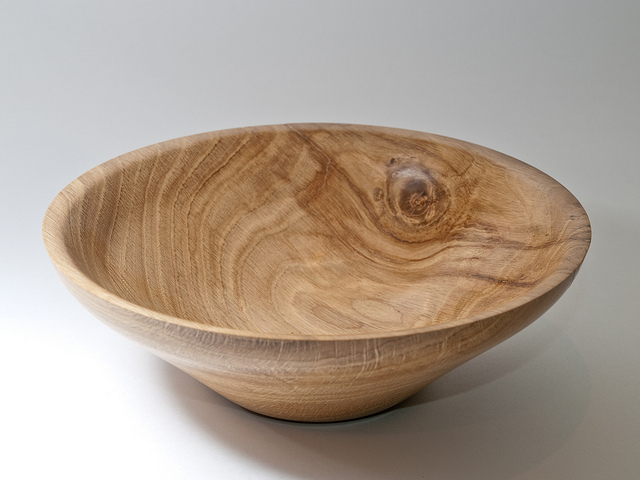
\includegraphics[scale=0.32]{images/Large-Bowl.jpg}
	\caption[Large Bowl]{Large Bowl \cite{fig:largeBowl}}
	\label{fig:largeBowl}
	\end{figure}

A random position on the surface of the bowl is the cost of the current values of the coefficients (cost). \\

The bottom of the bowl is the cost of the best set of coefficients, the minimum of the function.
The goal is to continue to try different values for the coefficients, evaluate their cost and select new coefficients that have a slightly better (lower) cost. \\

Repeating this process enough times will lead to the bottom of the bowl and you will know the values of the coefficients that result in the minimum cost. \cite{desc:GradientDescent}

\subsubsection{Method}


Gradient descent is based on the observation that if the multi-variable function
\(F(\mathbf {x} ) \) is defined and differentiable in a neighbourhood of a point \({\displaystyle \mathbf {a} } \) , 
then \( {\displaystyle F(\mathbf {x} )} \) decreases fastest if one goes from \({\displaystyle \mathbf {a} } \) in the direction of the negative gradient of \({\displaystyle F} \) at \( {\displaystyle \mathbf {a} }\) ,\( {\displaystyle -\nabla F(\mathbf {a} )} \). It follows that, if

\[ {\displaystyle \mathbf {b} =\mathbf {a} -\gamma \nabla F(\mathbf {a} )} \mathbf {b} =\mathbf {a} -\gamma \nabla F(\mathbf {a} ) \]

for \({\displaystyle \gamma }\)   small enough, then $ \displaystyle F(\mathbf {a}) \geq F(\mathbf {b}) $. In other words, the term \({\displaystyle \gamma \nabla F(\mathbf {a} )} \) is subtracted from $ \mathbf {a} $  because we want to move against the gradient, namely 
down toward the minimum. With this observation in mind, one starts with a guess $ \mathbf {x} _{0} $ for a local minimum of  $ F $, and considers the sequence $ \mathbf {x} _{0},\mathbf {x} _{1},\mathbf {x} _{2},\dots $ such that

\[ \mathbf {x} _{n+1}=\mathbf {x} _{n}-\gamma _{n}\nabla F(\mathbf {x} _{n}),\ n\geq 0. \]

We have

\[ F(\mathbf {x} _{0})\geq F(\mathbf {x} _{1})\geq F(\mathbf {x} _{2})\geq \cdots , \]

so hopefully the sequence  $ (\mathbf {x} _{n}) $ converges to the desired local minimum. Note that the value of the step size $ \gamma  $ is allowed to change at every iteration. With certain assumptions on the function $ F $ (for example,  F convex and $ \nabla F $ Lipschitz) and particular choices of  $ \gamma  $ (e.g., chosen either via a line search that satisfies the Wolfe conditions or the Barzilai-Borwein method shown as following),

\[ {\displaystyle \gamma _{n}={\frac {(\mathbf {x} _{n}-\mathbf {x} _{n-1})^{T}[\nabla F(\mathbf {x} _{n})-\nabla F(\mathbf {x} _{n-1})]}{||\nabla F(\mathbf {x} _{n})-\nabla F(\mathbf {x} _{n-1})||^{2}}}} \]

convergence to a local minimum can be guaranteed. When the function $ F $ is convex, all local minima are also global minima, so in this case gradient descent can converge to the global solution.

This process is illustrated in the adjacent picture. Here $ F $ is assumed to be defined on the plane, and that its graph has a bowl shape. The blue curves are the contour lines, that is, the regions on which the value of $ F $ is constant. A red arrow originating at a point shows the direction of the negative gradient at that point. Note that the (negative) gradient at a point is orthogonal to the contour line going through that point. We see that gradient descent leads us to the bottom of the bowl, that is, to the point where the value of the function $ F $ is minimal.
\cite{wiki:gradientDescent}

\section{Particle Swarm Optimization}
\textbf{Particle swarm optimization (PSO)} is a computational method that optimizes a problem by iteratively trying to improve a candidate solution with regard to a given measure of quality. It solves a problem by having a population of candidate solutions, here dubbed particles, and moving these particles around in the search-space according to simple mathematical formulae over the particle's position and velocity. Each particle's movement is influenced by its local best known position, but is also guided toward the best known positions in the search-space, which are updated as better positions are found by other particles. This is expected to move the swarm toward the best solutions. \\


PSO is a metaheuristic as it makes few or no assumptions about the problem being optimized and can search very large spaces of candidate solutions. However, metaheuristics such as PSO do not guarantee an optimal solution is ever found. More specifically, PSO does not use the gradient of the problem being optimized, which means PSO does not require that the optimization problem be differentiable as is required by classic optimization methods such as gradient descent and quasi-newton methods. \\

Formally, let $ f: \mathbb{R}^{n} \gets \mathbb{R} $ be the cost function which must be minimized. The function takes a candidate solution as argument in the form of a vector of real numbers and produces a real number as output which indicates the objective function value of the given candidate solution. The gradient of f is not known. The goal is to find a solution a for which $ f(a) \leq f(b) $ for all b in the search-space, which 
would mean a is the global minimum. Maximization can be performed by considering the function $ h = -f $ instead.
Let S be the number of particles in the swarm, each having a position $ x_{i} \in \mathbb{R}^{n} $ in the search-space and a velocity $ v_{i} \in \mathbb{R}^{n} $. Let pi be the best known position of particle i and let g be the best known position of the entire swarm. A basic PSO algorithm is then:

\newpage

\begin{algorithm}
	\caption{Basic PSO algorithm}\label{algo:pso}
	\begin{algorithmic}[1]
		\For{each particle i = 1, ..., S}
		\State Initialize the particle's position with a random vector: $ x_{i} \sim U(b_{lo}, b_{up}) $
		\State Initialize the particle's best known position to its initial position: $ p_{i} \gets x_{i} $
		\If{$ f(p_{i}) < f(g) $}
		\State update the swarm's best known  position: $ g \gets p_{i} $
		\EndIf
		\State Initialize the particle's velocity: $ v_{i} \sim  U(-|b_{up}-b_{lo}|, |b_{up}-b_{lo}|) $
		\While{a termination criterion is not met}
		\For{each particle $ i = 1, ..., S $}
		\For{each dimension $ d = 1, ..., n $}
		\State Pick random numbers: $ r_{p}, r_{g} \sim U(0,1) $
		\State          Update particle's velocity: $ v_{i,d} \gets \omega\, v_{i,d} + \phi_{p} r_{p} (p_{i,d}-x_{i,d}) + \phi_{g} r_{g} (g_{d}-x_{i},d) $
		\State Update the particle's position: $ x_{i} \gets x_{i} + v_{i} $
		\If{$ f(x_{i}) < f(p_{i}) $}
		\State Update the particle's best known position: $ p_{i} ← x_{i} $
		\If{$ f(p_{i}) < f(g) $}
		\State Update the swarm's best known position: $ g \gets p_{i} $
		\EndIf
		\EndIf
		\EndFor
		\EndFor
		\EndWhile
		\EndFor
	\end{algorithmic}
\end{algorithm}

The values $ b_{lo} $ and $ b_{up} $ are respectively the lower and upper boundaries of the search-space. The termination criterion can be number of iterations performed, or a solution with adequate objective function value is found. The parameters \omega, \phi p, and \phi g are selected by the practitioner and control the behaviour and efficacy of the PSO method. \cite{wiki:pso}
\newpage


\section{Differential Evolution}
n evolutionary computation, differential evolution (DE) is a method that optimizes a problem by iteratively trying to improve a candidate solution with regard to a given measure of quality. Such methods are commonly known as metaheuristics as they make few or no assumptions about the problem being optimized and can search very large spaces of candidate solutions. However, metaheuristics such as DE do not guarantee an optimal solution is ever found. \\

DE is used for multidimensional real-valued functions but does not use the gradient of the problem being optimized, which means DE does not require for the optimization problem to be differentiable as is required by classic optimization methods such as gradient descent and quasi-newton methods. DE can therefore also be used on optimization problems that are not even continuous, are noisy, change over time, etc. \\

DE optimizes a problem by maintaining a population of candidate solutions and creating new candidate solutions by combining existing ones according to its simple formulae, and then keeping whichever candidate solution has the best score or fitness on the optimization problem at hand. In this way the optimization problem is treated as a black box that merely provides a measure of quality given a candidate solution and the gradient is therefore not needed. \\

DE is originally due to Storn and Price. Books have been published on theoretical and practical aspects of using DE in parallel computing, multiobjective optimization, constrained optimization, and the books also contain surveys of application areas. \cite{wiki:de}

\subsubsection{Basics}
DE is a very simple population based, stochastic function minimizer which is very powerful at the same time. DE managed to finish 3rd at the First International Contest on Evolutionary Computation (1s tICEO) which was held in Nagoya, may 1996. DE turned out to be the best genetic type of algorithm for solving the real-valued test function suite of the 1st ICEO (the first two places were given to non-GA type algorithms which are not universally applicable but solved the test-problems faster than DE). The crucial idea behind DE is a scheme for generating trial parameter vectors. \\

\newpage 
The flowchart of DE as follows,
\vspace{30px}
	\begin{figure}[!bth]
	\center
	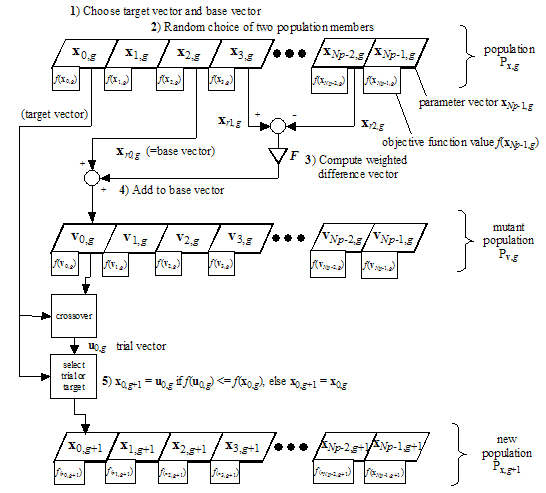
\includegraphics[scale=1.2]{images/de2.jpg}
	\caption[Flowchart of Differential Evolution]{Flowchart of Differential Evolution \cite{diag:de}}
	\label{fig:deFlowchart}
	\end{figure}

\newpage

\section{Fireworks Algorithm}
Setting off fireworks is an important creative and joyful activity during Spring Festival in China. At this time, tens of thousands of fireworks explode in the night sky and show beautiful patterns of sparks. Usually, fireworks of different prices and specifications produce entirely different patterns. For example, fireworks of lower price produce less sparks with larger amplitude compared with higher price fireworks and vice versa. The way fireworks explode is similar to the way an individual searches the optimal solution in swarm intelligence algorithms. As a swarm intelligence algorithm, fireworks algorithm consists of four parts, i.e., the explosion operator, mutation operator, mapping rule and selection strategy. The effect of the explosion operator is to generate sparks around fireworks. The number and amplitude of the sparks are governed by the explosion operator. After that, some sparks are produced by mutation operator. The mutation operator utilizes Gaussian operator to produce sparks in Gaussian distribution. Under the effect of the two operators, if the produced spark is not in the feasible region, the mapping rule will map the new generated sparks into the feasible region. To select the sparks for next generation, the selection strategy is used. Fireworks algorithm runs iteratively until it reaches the termination conditions.

\subsection{FA Framework}

When a firework is set off, a shower of sparks will fill the local space around thefirework. In our opinion, the explosion process of a firework can be viewed asa search in the local space around a specific point where the firework is set offthrough the sparks generated in the explosion. When we are asked to find a pointxjsatisfying $ f(x_{j})=y $, we can continually set off ‘fireworks’ in potential spaceuntil one ‘spark’ targets or is fairly near the point xj. Mimicking the process ofsetting off fireworks, a rough framework of the FA is depicted in \ref{fig:FAFramework}. \\

In the FA, for each generation of explosion, we first select \textit{n} locations, where \textit{n} fireworks are set off. Then after explosion, the locations of sparks are obtained and evaluated. When the optimal location is found, the algorithm stops. Otherwise, \textit{n} other locations are selected from the current sparks and fireworks for the next generation of explosion.
\\
From \ref{fig:FAFramework}, it can be seen that the success of the FA lies in a good design
of the explosion process and a proper method for selecting locations, which are
respectively elaborated in the further subsections.

\newpage
	\begin{figure}[!bth]
	\center
	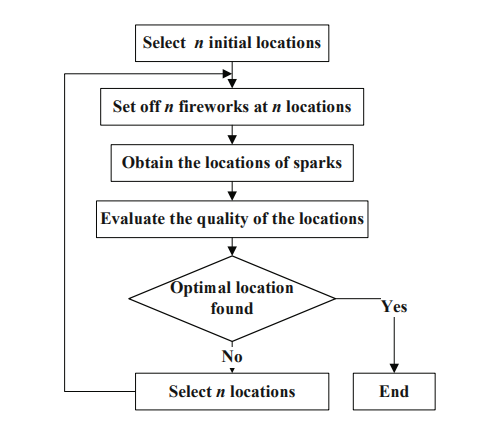
\includegraphics[scale=0.5]{images/FA_flowchart.png}
	\caption[Framework of fireworks algorithm]{Framework of fireworks algorithm \cite{paper:fwa}}
	\label{fig:FAFramework}
	\end{figure}

\subsection{Design of Fireworks Explosion}
Through observing fireworks display, we have found two specific behavior of
fireworks explosion. When fireworks are well manufactured, numerous sparks are
generated, and the sparks centralize the explosion center. In this case, we enjoy
the spectacular display of the fireworks. However, for a bad firework explosion,
quite few sparks are generated, and the sparks scatter in the space. \\

The two manners are depicted in \ref{fig:FWAtypesofexplosion}. From the standpoint of a search
algorithm, a good firework denotes that the firework locates in a promising area
which may be close to the optimal location. Thus, it is proper to utilize more
sparks to search the local area around the firework. In the contrast, a bad firework
means the optimal location may be far from where the firework locates. Then,
the search radius should be larger. In the FA, more sparks are generated and
the explosion amplitude is smaller for a good firework, compared to a bad one.

	\begin{figure}[!bth]
	\center
	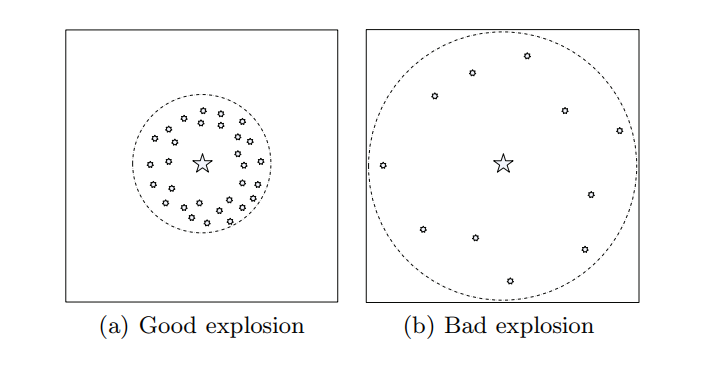
\includegraphics[scale=0.5]{images/typesOfFireworksExplosion.png}
	\caption[Two types of fireworks explosion]{Two types of fireworks explosion \cite{paper:fwa}}
	\label{fig:FWAtypesofexplosion}
\end{figure}

\newpage

\textbf{Number of Sparks.} Suppose the FA is designed for the general optimization
problem:
	\begin{equation}
	\label{eq:minimizefx}
	 Minimize f(x) \in \mathbb{R}, x_{min} \leq x \leq x_{max} ,
	\end{equation}
	
	where $ x = x_{1}, x_{2},...,x_{d} $ denotes a location in the potential space, $ f(x) $ is an
	objective function, and $ x_{min} $ and $ x_{max}  $ denote the bounds of the potential space.
	Then the number of sparks generated by each firework $ x_{i} $ is defined as follows.
	\begin{equation}
	\label{eq:noOfSpark}
		s_{i} = m \cdot \dfrac{y_{max} - f(x_{i}) + \epsilon }{\sum_{n}^{i = 1} (y_{max} - f(x_{i})) + \epsilon}
	\end{equation}
	
	where m is a parameter controlling the total number of sparks generated by
	the n fireworks, $ y_{max} = max(f(x_{i})) (i = 1, 2,...,n) $ is the maximum (worst)
	value of the objective function among the \textit{n} fireworks, and \epsilon, which denotes the
	smallest constant in the computer, is utilized to avoid zero-division-error.
	To avoid overwhelming effects of splendid fireworks, bounds are defined for
	$ s_{i} $, which is shown in \ref{eq:limitSparks}.
	
	\begin{equation}
	\label{eq:limitSparks}
		\hat{s_{i}} =  \Bigg\{
		\begin{tabular}{cc}
		round(a \cdot m) & $ if s_{i} < am $ \\
		round(b \cdot m) & if $ s_{i}  > bm , a < b < 1 \,$,\\
		round($ s_{i} $) & otherwise \\
		\end{tabular}
	\end{equation}
	where \textit{a} and \textit{b} are const parameters.

\newpage
	
	\textbf{Amplitude of Explosion.} In contrast to the design of sparks number, the amplitude
	of a good firework explosion is smaller than that of a bad one. Amplitude
	of explosion for each firework is defined as follows.
	
	\begin{equation}
		A_{i} = \hat{A} \cdot \frac{f(x_{i}) - y_{min} + \epsilon}{\sum_{n}^{i = 1}(f(x_{i}) - y_{min}) + \epsilon} ,
	\end{equation}
	where $ \hat{A} $ denotes the maximum explosion amplitude,and $ y_{min} = min(f(x_{i})) (i =
	1, 2,...,n) $ is the minimum (best) value of the objective function among the \textit{n}
	fireworks.
	
	
	\begin{algorithm}
		\caption{Obtain the location of a spark}\label{algo:fwaLocationofSpark}
		\begin{algorithmic}[0]
		\State Initialize the location of the spark: $ \tilde{x}_{j} = x_{i} $ ;
		\State $ z = round(d \cdot rand(0, 1)) $;
		\State Randomly select $ z $ dimensions of $ \tilde{x}_{j} $;
		\State Calculate the displacement: $ h = A_{i} \cdot rand(−1, 1) $;
		\For{each dimension $ \tilde{x}_{k}^{j} \in $ \{ pre-selected \textit{z} dimensions of $ \tilde{x}_{j} $ \}}
		\State $ \tilde{x}_{k}^{j} = \tilde{x}_{k}^{j} + h $;
		\If{$ \tilde{x}_{k}^{j} < \tilde{x}_{min}^{j} $ or $ \tilde{x}_{k}^{j} > \tilde{x}_{k}^{max} $}
		\State map $ \tilde{x}_{k}^{j} $ to potential space: $ \tilde{x}_{k}^{j} = \tilde{x}_{k}^{min} + | \, \tilde{x}_{k}^{j} \, | \, \%(\tilde{x}_{k}^{max} - \tilde{x}_{k}^{min}) $;
		\EndIf
		\EndFor
		\end{algorithmic}
	\end{algorithm}

	\begin{algorithm}
	\caption{ Obtain the location of a specific spark}
	\label{algo:fwaLocationOfSpecificSpark}
	\begin{algorithmic}[0]
		\State Initialize the location of the spark: $ \tilde{x}_{j} = x_{i} $ ;
		\State $ z = round(d \cdot rand(0, 1)) $;
		\State Randomly select $ z $ dimensions of $ \tilde{x}_{j} $;
		\State Calculate the coefficient of Gaussian explosion: $ g $ = Gaussian(1, 1);
		\For{each dimension $ \tilde{x}_{k}^{j} \in $ \{ pre-selected \textit{z} dimensions of $ \tilde{x}_{j} $ \}}
		\State $ \tilde{x}_{k}^{j} = \tilde{x}_{k}^{j} \cdot g $;
		\If{$ \tilde{x}_{k}^{j} < \tilde{x}_{min}^{j} $ or $ \tilde{x}_{k}^{j} > \tilde{x}_{k}^{max} $}
		\State map $ \tilde{x}_{k}^{j} $ to potential space: $ \tilde{x}_{k}^{j} = \tilde{x}_{k}^{min} + | \, \tilde{x}_{k}^{j} \, | \, \%(\tilde{x}_{k}^{max} - \tilde{x}_{k}^{min}) $;
		\EndIf
		\EndFor
	\end{algorithmic}
\end{algorithm}


	\begin{algorithm}
	\caption{ Framework of the FA}
	\label{algo:fwaFramework}
	\begin{algorithmic}[0]
		\State Randomly select $ n $ locations for fireworks;
		\While{stop criteria = false}
		\State Set off $ n $ fireworks respectively at the $ n $ locations:
		\For{each firework $ x_{i} $}
		\State Calculate the number of sparks that the firework yields: $ \tilde{S}_{i} $, according to Eq.\ref{eq:limitSparks}
		\State Obtain locations of $ \tilde{S}_{i} $ sparks of the firework $ x_{i} $ using Algorithm \ref{algo:fwaLocationofSpark}
		\EndFor
		\For{$ k = 1:\hat{m} $}
		\State Randomly select a firework $ x_{j} $ ;
		\State Generate a specific spark for the firework using Algorithm \ref{algo:fwaLocationOfSpecificSpark};
		\EndFor
		\State Select the best location and keep it for next explosion generation;
		\State Randomly select n − 1 locations from the two types of sparks and the current
			fireworks according to the probability;
		\EndWhile
	\end{algorithmic}
\end{algorithm}
	
\newpage


%The table \ref{table:3} is an example of referenced \LaTeX elements in landscape.
%
%\begin{landscape}
%
%\begin{table}[bth]
%\begin{center}
%\caption{Table to test captions and labels}
%\label{table:3}
%\begin{tabular}{ |c| c| c| }
%\hline
% cell1 & cell2 & cell3 \\ 
% \hline
% cell4 & cell5 & cell6 \\ 
% \hline 
% cell7 & cell8 & cell9   \\ 
% \hline
%\end{tabular}
%
%\end{center}
%\end{table}
%
%\end{landscape}

\newpage

\chapter{Results \& Discussion}

\section{Data Set Information}

\subsection{Concrete Slump Test}
\begin{tabular}{l l}
	Data Set Characteristics:  & Multivariate \\
	Associated Tasks: & Regression  \\
	Attribute Characteristics: & Real \\
	Number of Instances: & 103 \\
	Number of Attributes: & 10 \\
\end{tabular}

\subsection{Housing Data Set}
\begin{tabular}{l l}
	Data Set Characteristics:  & Multivariate \\
	Associated Tasks: & Regression  \\
	Attribute Characteristics: & Categorical, Integer, Real \\
	Number of Instances: & 506 \\
	Number of Attributes: & 14 \\
\end{tabular}

\subsection{Challenger USA Space Shuttle O-Ring Data Set }
\begin{tabular}{l l}
	Data Set Characteristics:  & Multivariate \\
	Associated Tasks: & Regression  \\
	Attribute Characteristics: & Integer \\
	Number of Instances: & 23 \\
	Number of Attributes: & 4 \\
\end{tabular}

\subsection{Concrete Compressive Strength Data Set}
\begin{tabular}{l l}
	Data Set Characteristics:  & Multivariate \\
	Associated Tasks: & Regression  \\
	Attribute Characteristics: & Real \\
	Number of Instances: & 1030 \\
	Number of Attributes: & 9 \\
\end{tabular}

\subsection{Red Wine Quality Data Set}
\begin{tabular}{l l}
	Data Set Characteristics:  & Multivariate \\
	Associated Tasks: & Classification, Regression  \\
	Attribute Characteristics: & Real \\
	Number of Instances: & 1599 \\
	Number of Attributes: & 12 \\
\end{tabular}

\subsection{White Wine Quality Data Set}
\begin{tabular}{l l}
	Data Set Characteristics:  & Multivariate \\
	Associated Tasks: & Classification, Regression  \\
	Attribute Characteristics: & Real \\
	Number of Instances: & 4898 \\
	Number of Attributes: & 12 \\
\end{tabular}

\section{Parameter Settings}
\subsection{Gradient Descent}
\begin{tabular}{l l}
	Learning Rate \alpha: & 0.6 \\
	Number of function evaluations: & 2000 \\ 
\end{tabular}

\subsection{Particle Swarm Optimization}
\begin{tabular}{l l}
	Number of particles: & 10 \\
	Number of function evaluations: & 2000 \\ 
	Inertia weight = & 0.729 \\
	c1, c2 = & 1.44945 \\
	$ x_{max} $ = & 1 \\
	$ x_{min} $ = & 0 \\
\end{tabular}

\subsection{Differential Evolution}
\begin{tabular}{l l}
	Population \textit{N} : & 10\\
	Number of function evaluations: & 2000 \\ 
	Crossover Rate: & 0.8 \\
	Scale Factor: & 0.9 \\
\end{tabular}

\subsection{Fireworks}
\begin{tabular}{l l}
	Initial Population (\textit{N}) : & 10\\
	Number of function evaluations: & 2000 \\ 
	\textit{a}: & 0.04 \\
	\textit{b}: & 0.8 \\
	$ \hat{m} $: & 10 \\
	\textit{m}: & 50 \\
	Maximum Amplitude ($ \hat{A} $): & 40 \\
\end{tabular}

\newpage

\subsection{Results}
\subsubsection{Training Set}

\begin{table}[!htbp]
	\centering
	\caption{Result Table}
	\label{tab:ResultTable}
	\sisetup{round-mode=places,round-precision=4} 
\begin{tabular}{@{}lSSlSSl@{}}
	\toprule
	Datasets                              & \multicolumn{3}{c}{GD}                           & \multicolumn{2}{c}{PSO}              &         \\ \midrule
	& \text{Mean}              & \text{Std}               & \text{Time}     & \text{Mean}             & \text{Std}               & \text{Time}    \\
	Slump Test                            & 2.11575119732343  & 0.109342267127141 & 3.40E-05 & 9.12803953216337 & 0.422076958348553 & 1.5E-05 \\
	Housing Dataset                       & 29.2290820008102  & 1.09103095261502  & 1.5E-05  & 36.314726113291  & 2.15992764536123  & 1.6E-05 \\
	O-ring Dataset                        & 0.002144357727271 & 0.011384143971044 & 1.5E-05  & 23.1369782424306 & 2.06071867218733  & 2.4E-05 \\
	Concrete Dataset & 83.9624336397099  & 1.17531980535434  & 1.4E-05  & 88.7812657199354 & 0.997033380502257 & 3.6E-05 \\
	Red Wine Quality                      & 128.156212682023  & 1.38911792157694  & 1.4E-05  & 139.684735932487 & 1.94112172925811  & 1.6E-05 \\
	White Wine Quality                    & 380.693571742112  & 2.56592649760963  & 1.4E-05  & 440.368621857887 & 6.44617981000869  & 2E-05  
\end{tabular}
\end{table}

\begin{table}[!htbp]
	\centering
	\caption{Continuation of Result Table}
	\label{tab:ResultTableCont}
	\sisetup{round-mode=places,round-precision=4} 
	\begin{tabular}{@{}lSSlSSl@{}}
		\toprule
		Datasets           & \multicolumn{3}{c}{DE}                         & \multicolumn{3}{c}{FWA}                         \\ \midrule
		& \text{Mean}             & \text{Std}              & \text{Time}     & \text{Mean}             & \text{Std}               & \text{Time}     \\
		Slump Test         & 8.24659237311693 & 2.74694162223394 & 0.018889 & 16.6107653437399 & 0.613809306739308 & 3.695438 \\
		Housing Dataset    & 58.8853873030071 & 2.72842625333641 & 0.075811 & 44.653822098153  & 2.72842625333641  & 3.410051 \\
		O-ring Dataset     & 0.03666783748193 & 1.75438567105428 & 0.018523 & 57.1095959596118 & 1.75438567105428  & 3.524133 \\
		Concrete Dataset   & 86.7841713943101 & 5.05542081881594 & 0.075699 & 97.2449368583716 & 5.05542081881594  & 3.110807 \\
		Red Wine Quality   & 141.970706333197 & 4.26518935825816 & 0.065636 & 142.236598083891 & 4.26518935825816  & 3.853955 \\
		White Wine Quality & 409.223840576782 & 4.01944402137273 & 0.129604 & 406.197996776574 & 4.01944402137273  & 4.339977
	\end{tabular}
\end{table}

\subsection{Discussion}
From the above Table \ref{tab:ResultTable} and \ref{tab:ResultTableCont} it can be seen that for almost all the data sets Gradient Descent Chapter.\ref{chap:GD} trumps all of the other algorithms. The error is the lowest of all the other algorithms. Also the runtime complexity is several magnitude lower for the same 2000 function evaluations. Also the standard deviation is lowest among them. That signifies robustness. 


\newpage

\chapter{Conclusions}
In the above pages, 4 different algorithms (Gradient Descent, Particle Swarm Optimization, Differential Evolution, Fireworks Algorithm) are compared against 5 data sets. It is found that despite having simplest implementation and technique, Gradient Descent performs best among the rest of the algorithms. It is also more efficient, more robust and have less complexity.

\newpage
\begin{thebibliography}{50}
	
\bibitem{desc:RegressionAnalysis}
\url{https://www.analyticsvidhya.com/blog/2015/08/comprehensive-guide-regression}

\bibitem{wiki:LinearRegression}
\url{https://en.wikipedia.org/wiki/Linear_regression}

\bibitem{desc:RegressionApplication}
\url{http://smallbusiness.chron.com/application-regression-analysis-business-77200.html}

\bibitem{desc:GradientDescent}
\url{http://machinelearningmastery.com/gradient-descent-for-machine-learning/}

\bibitem{fig:largeBowl}
\href{https://www.flickr.com/photos/wwarby/4046737583/}{William Warby}

\bibitem{wiki:gradientDescent}
\url{https://en.wikipedia.org/wiki/Gradient_descent}

\bibitem{wiki:pso}
\url{https://en.wikipedia.org/wiki/Particle_swarm_optimization}

\bibitem{diag:de}
\url{http://www1.icsi.berkeley.edu/~storn/code.html}

\bibitem{wiki:de}
\url{https://en.wikipedia.org/wiki/Differential_evolution}

\bibitem{paper:fwa}
Y. Tan, and Y. Zhu, Firework Algorithm for Optimization, In: Y. Tan et
al.(Eds): ICSI 2010, Part I, LNCS 6145, pp.355–364, 2010, Springer-
Verlag Berlin Heidelberg 2010.

\end{thebibliography}


\end{document}
